\chapter{克服拖延症} % Introduction chapter suppressed from the table of contents


技术总监问:现在我遇到最大的难题就是如何提升下面技术人员的能力,如果他们全都是高手,我就很轻松了,但实际上高手最多只有1/3,其他都是中低水平。你接触过这么多软件开发团队,有什么好方案?\\
我:你可以先听听以下故事。\\

\begin{description}
\tightlist
\item[]
= = = = = = = = = =
\end{description}

小李:你平常办公时间一直都很忙,还可以腾出晚上和周末时间,把客户遇到的问题,如何解决等,汇总成分享文章,每两周公众号发布,很厉害呀。\\
我:其实你也可以做到。要成为专业软件工程师,除了要学习软件工程相关的知识与技能外,个人有没有高效率的习惯其实更重要。\\
我在5年前教项目管理时参考过一本效率小册(详见参考Reference),这本小册罗列了99个小技巧,每个技巧都不超过一页纸,我自己也一直用这小手册提醒自己。\\ 

%\url{文件:超效率目录.png}

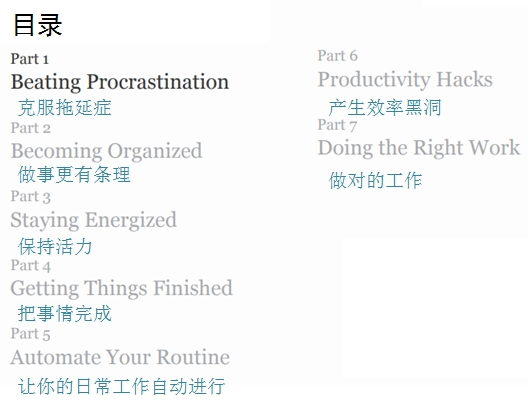
\includegraphics[width=6cm]{Screenshotfrom2023-10-1523-05-0011.jpg}

例如,第一章克服拖延症,这里的内容几乎全部都有帮助。\\



\hypertarget{ux6839ux56e0ux5206ux6790ux8befux89e3ux6848ux4f8b}{%
\subsubsection{周/日目标 (Weekly/ Daily Goals)}\label{ux6839ux56e0ux5206ux6790ux8befux89e3ux6848ux4f8b}}

\framebox{%
\begin{minipage}[t]{0.97\columnwidth}\raggedright
我每天都会订计划,早上希望完成哪些功能,下午完成哪些。当然这个计划也会按实际的进展调整。

周 /
日目标是个人时间管理的基本功。每一天第一件事不是回邮件,而是仔细想想今天要完成什么任务,每一周的开始,也应该想我本周希望完成什么任务。不然的话,每天的时间就很容易被琐碎的小事吃掉,一事无成。\\
\strut
\end{minipage}}

\framebox{%
\begin{minipage}[t]{0.97\columnwidth}\raggedright
背后体现的道理很简单, 要把时间花在重要、但非紧急的活动上,效率才会体现出来。

%\href{文件:紧迫非紧迫_3.0.png}{600px}
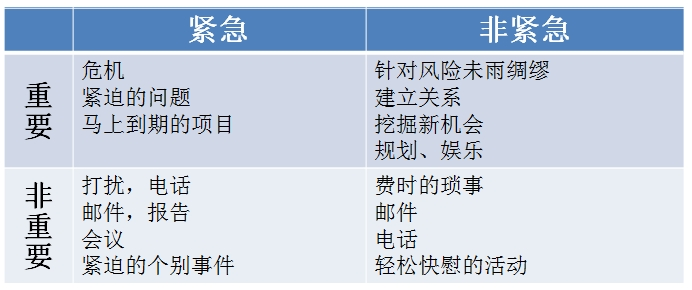
\includegraphics[width=6cm]{紧急非紧急.jpg}

\strut
\end{minipage}}

\hypertarget{ux6839ux56e0ux5206ux6790ux8befux89e3ux6848ux4f8b}{%
\subsubsection{限定时间 (Timeboxing)}\label{ux6839ux56e0ux5206ux6790ux8befux89e3ux6848ux4f8b}}

\framebox{%
\begin{minipage}[t]{0.97\columnwidth}\raggedright
 把每天的任务安排成时间段,每一段不应超过1.5小时。\\ 
一般人可以专心集中的时间段都不会超过60分钟,小孩可能更短。如果老师叫你星期五5点钟交卷,你不会提前交,都会等到最后10分钟,甚至最后5分钟。所以如果我们把一天的时间切开,分成
1~1.5小时时间段,自然有动力,希望在时间之内完成任务。\\
我们写代码的时候应该也是用同样的原理。例如某些编程活动尝试了多次,但没有进展,有时总共会花超过10小时。所以每次当我发现某编程工作超过了2小时,我就会先做其他事情。\strut
\end{minipage}}


\hypertarget{ux6839ux56e0ux5206ux6790ux8befux89e3ux6848ux4f8b}{%
\subsubsection{分解任务 (Dissolving tasks)}\label{ux6839ux56e0ux5206ux6790ux8befux89e3ux6848ux4f8b}}

\framebox{%
\begin{minipage}[t]{0.97\columnwidth}\raggedright
个人学习编程经验:因为都是练习题,所以每一个功能都比较细,不会超过20 行。如果我们平常做开发时,也必须要把一些大、复杂的功能预先细分才有效率。
\strut
\end{minipage}}


\hypertarget{ux6839ux56e0ux5206ux6790ux8befux89e3ux6848ux4f8b}{%
\subsubsection{加强自律 (Building Self-Discipline Muscles)}\label{ux6839ux56e0ux5206ux6790ux8befux89e3ux6848ux4f8b}}


\hypertarget{ux6839ux56e0ux5206ux6790ux8befux89e3ux6848ux4f8b}{%
\subsubsection{晨礼(Morning Rituals) 日常运动 (Make an Exercise Routine)}\label{ux6839ux56e0ux5206ux6790ux8befux89e3ux6848ux4f8b}}


\framebox{%
\begin{minipage}[t]{0.97\columnwidth}\raggedright
不要以为编码是一个单纯的脑力活,整天坐在屏幕前面敲代码就可以。如果人的体力、精力没有配合上也会出问题,好在我每天早上一直坚持30
\textasciitilde{}
40分钟的轻量运动,然后晚饭前0.5 ~ 1小时的骑单车或者慢跑的习惯。中间也不是整天坐着,一段时间会走一走、喝点儿橙汁等,以确保身体不断在动,这样才不会困,保持动力。

贝多芬每天都会通过去外面散步来获得一些创作的灵感,然后他会立马把这些写在本子上,用于后面的音乐创作。
\strut
\end{minipage}}

我:身体健康,精神状态也同样重要,你每周有锻炼的习惯吗?\\
小李:没有,每天都太忙了,虽然一直觉得身体不如几年前了,也知道锻炼好,但无法抽出时间。\\
我:我也很忙,但深知定期运动对身体非常重要,我一直按以下2种方法保持个人身体状态--

\begin{itemize}
\tightlist
\item
  工作时尽量避免长期坐下来,因我主要做培训、咨询、评估,所以可以大部分时间站着或在走动。(NEAT\#)。
\item
  尽量每天7点吃早餐前跑圈,疾跑1.5 ~ 
  2分钟,休息半分钟,重复这循环4~6轮。(HIIT\#)。
\end{itemize}

\hypertarget{ux6839ux56e0ux5206ux6790ux8befux89e3ux6848ux4f8b}{%
\subsubsection{不会分心的工作场所 (Create a Distraction-Free workplace)}\label{ux6839ux56e0ux5206ux6790ux8befux89e3ux6848ux4f8b}}

\hypertarget{ux6839ux56e0ux5206ux6790ux8befux89e3ux6848ux4f8b}{%
\subsubsection{轻策划、迭代、再策划 (Ready , Fire, Aim!)}\label{ux6839ux56e0ux5206ux6790ux8befux89e3ux6848ux4f8b}}

\framebox{%
\begin{minipage}[t]{0.97\columnwidth}\raggedright
30年前,软件开发都是一些大型的项目,整个架构要设计好才动手去写代码。现在反过来,需求变化极大,开发都需要敏捷,轻文档、轻计划,尽尽快写好代码,做一些功能给客户,从反馈优化下一轮。我这次的几天开发也是用同样原则,没有花时间在一些设计或者文档。想直接把代码写出来,并通过单元测试,节省了很多耗时间的工作。把有限的时间都放在写好代码上。
\strut
\end{minipage}}


\hypertarget{ux6839ux56e0ux5206ux6790ux8befux89e3ux6848ux4f8b}{%
\subsubsection{不断清洗 (Churning)}\label{ux6839ux56e0ux5206ux6790ux8befux89e3ux6848ux4f8b}}

\framebox{%
\begin{minipage}[t]{0.97\columnwidth}\raggedright
万事起头难。我假期重学编码时也是遇到同样问题,不知如何入手,太久没看写代码的书了,很多基本的都不知如何入手。所以我开始的时候不会直接尝试写题目里面的功能,而是重写一些书本的代码,看看结果怎么样,然后逐步提升。写一些基本功能,慢慢有了习惯,调整过来了,后面就越来越顺。好比一台旧的水泵,刚开始抽上来的水总是有难喝的铁锈,只要不停止抽水,当污水最终都从系统中抽出后,就能发现底下的净水。
\strut
\end{minipage}}

\hypertarget{ux6839ux56e0ux5206ux6790ux8befux89e3ux6848ux4f8b}{%
\subsubsection{要有好的土壤 (Remove your Hidden Roadblocks)}\label{ux6839ux56e0ux5206ux6790ux8befux89e3ux6848ux4f8b}}

\framebox{%
\begin{minipage}[t]{0.97\columnwidth}\raggedright
在含盐量高的土壤里种植物是结不出果实的。浇水、平衡在阴凉处和阳光下的时间都抵不过根部吸入的毒素。如果我们没有积极性,就可能是土壤的问题。如果没有足够的积极动力,就不会在长假专注写程序,也不会定期要求自己写分享文章。所以要有明确、很想达到的目标驱动。
像作曲家希望写出很多经典的优秀作品一样,会不满足于现在的状态。觉得自己的灵感或者创造力没有发挥出来,成为可以保留下来的东西。也是这种驱动力让我可以一直努力做这件事。
\strut
\end{minipage}}


\hypertarget{ux6839ux56e0ux5206ux6790ux8befux89e3ux6848ux4f8b}{%
\subsubsection{摒弃拖延恶习 (Quit your Procrastination Vices)}\label{ux6839ux56e0ux5206ux6790ux8befux89e3ux6848ux4f8b}}

\framebox{%
\begin{minipage}[t]{0.97\columnwidth}\raggedright
长假里,大部分人都会把时间用于看视频或电视剧,而我正好没有这个习惯,也一直没有玩网络游戏的习惯,否则肯定完成不了。
\strut
\end{minipage}}

最终我用日程记录(Timelogging),把整件事和什么活动、时间花在什么地方都记录下来了。

小李:我看你上面列出的技巧,我大部分都还没做到。

我:不要紧,我6年前刚开始定期写文章时跟你一样,但只要不放弃,一直往既定目标努力,不良习惯最终都会改正过来。我常常说人的潜力是极大的。舒伯特你听过吗?\\
小李:好像是很有名的作曲家。\\
我:是的,但他31岁就去世了,你猜他一生一共写了多少首歌和音乐作品。\\
小李:我记得中学时,老师介绍过他的艺术作品,如《鳟鱼》,但他31岁就死了,我猜100 \textasciitilde{} 200 首歌?\\
我:他一生写了超过460首歌曲(时长\textgreater{}24小时)。除了歌曲,他还写了其他作品,如9首交响曲(1首未完成,1首只有草稿)、20
室内乐、120 钢琴曲等,每一类都包括大量经典作品,对后世影响深远。\\
小李:如果粗算一下,他一生约有600个作品,算他有16年时间作曲,平均每月要完成3个作品,真是不得了。\\
我:虽然他的作品有大有小(从一首歌到45分钟的交响曲),他确实生产率极高,而且他最后的7年身体一直都不好,所以他那个时候肯定不会像我们现代“996”方式工作。
他每天主要是早上用来写作,傍晚便去休息散步。但他会同时做多个创作项目。
如果项目没有灵感,就暂时放下来,创作其他作品。
他著名的未完成交响曲就是个好例子,只有两个乐章(一般交响曲都是4个乐章)。
所以他是使用高效技巧的一个成功例子。
每个人都有自己的理想,但如果没有高效率来执行,理想只是天马行空、天方夜谭,不会有任何成就。
除了以上这些技巧外,保持整洁也重要。你有没有试过想找某东西,找半天都找不着?

小李:确实经常发生,而且还会遗漏东西。我上次出差便忘记了iPhone,后面回北京后电话联系当地酒店前台后,我找当地同事去酒店取,然后快递给我,烦死了。\\
我:有听过5S (5S法\#)
吗?例如,如果你把东西都放固定地方,就可以避免同类问题再发生。如果你一直在一个很乱的环境工作,会导致心情烦躁,对工作、身体都不好。

\begin{description}
\item[]
\begin{description}
\tightlist
\item[]
(\#详见附件”锻炼之道”的多了解  NEAT、HIIT;5S法详见第1章附件。)
\end{description}
\end{description}

总监:我大概懂你的意思了,要提升技术人员的能力应先改变他们的习惯 —— 如时间管理,才有机会提升。\\

\begin{description}
\tightlist
\item[]
= = = = = = = =
\end{description}

总监:我大概懂你的意思了,要提升技术人员的能力先要改变他们的习惯,有良好的习惯--如时间管理,才有机会提升。\\

\framebox{%
\begin{minipage}[t]{0.97\columnwidth}\raggedright
即时笔记 (The Capture Device)\\
总监边听边在本子上记下那些重点。高效的人都会有工具帮他记录想到的灵感、想法、项目、待做事项等,不会仅仅靠大脑记忆。你提出一个要求,他会立马写在小本子上,你会觉得他应该会按你要求去处理,但反过来如他只是口头说会处理,你会担心很可能没有下文。但我看有些领导,身边只拿个手机,除非他们的记忆力超人,否则我估计他每天都会忘记不少重要事项。
\strut
\end{minipage}}

\hypertarget{ux7ed3ux675fux8bed}{%
\subsection{结束语}\label{ux7ed3ux675fux8bed}}

\framebox{%
\begin{minipage}[t]{0.97\columnwidth}\raggedright
很赞同杭州某高级经理的总结:\\
人一定要自律!你说的小技巧确实能起到很大帮助,而且我基本都会使用,但如果不养成习惯,想起来使用下,最终还是改不了拖延症。所以要解决拖延症,一定从根源做起,还是得靠自己,需要培养自己意志力、专注力,坚持好习惯,改掉坏毛病。
\strut
\end{minipage}}

我相信人分高低,但并非取决于基因、种族,主要取决于她后天的习惯、自律与努力。要养成良好习惯要从小开始,深受家庭和教育的影响,所以百年树人。

与公司改进一样,改变个人习惯很难,这些技巧可以帮助个人改善。

\hypertarget{ux9644ux4ef6}{%
\section{附件}\label{ux9644ux4ef6}}


\hypertarget{ux953bux70bcux4e4bux9053-the-truth-about-exercise}{%
\subsection{锻炼之道 The Truth about
EXERCISE}\label{ux953bux70bcux4e4bux9053-the-truth-about-exercise}}

想大家都同意和相信:
``多运动,便多烧耗卡路里,便能帮助减肥,降低体重。''

\framebox{%
\begin{minipage}[t]{0.97\columnwidth}\raggedright
某国家给市民的健康指南:每周起码做150分钟中强度锻炼,或75分钟高强度锻炼。
\strut
\end{minipage}}


但不是每个人都能每天抽时间做锻炼,有什么更好方法?\\
不一定只依赖去健身室锻炼,平常工作生活少坐多走、站着工作、开会,甚至小动作等都有帮助。

\framebox{%
\begin{minipage}[t]{0.97\columnwidth}\raggedright
N.E.A.T. (Non-exercise activity thermogenesis) 小实验;
教授使用有电子传感器的底裤,记录记者、咖啡厅女服务员、商务人员3人一周每天正常工作中消耗多少卡路里。\\
发现:

\begin{itemize}
\tightlist
\item
  女服务员最好。因每天都非常忙碌(尤其是早餐时段),送餐、接单、做咖啡等等。
\item
  商务人员第二。虽然有很多时间坐下来,但每天都会走一公里路见客户,而且每周二、五下班后会去健身锻炼。
\item
  记者最差。每天无论工作或家里,大部分时间都是坐下不动,所以他看起来不胖,但其实体内存有大量脂肪,集中在肝、肾等内脏。
\end{itemize}\strut
\end{minipage}}

这实验告诉我们:如果每天一直坐下不动很不好,就算每天下班后晚上都去健身锻炼也帮不了。

后面记者听教授建议,改变习惯,定期站起来走动。如与同事交流与尽量边走路边交流,减少长期坐下来;
多爬楼梯,少用电梯;骑单车,不开车等方式。
后面,从实验数据分析,发现这些改变帮他增加每天卡路里消耗接近一倍,到500水平。

研究发现不断大量健身锻炼不一定对每个人都有效。
有20\%会没有效果,另一端对15\%的人会非常有效。
这跟人的基因密切相关,所以多锻炼不一定都有效。

\begin{description}
\tightlist
\item[]
= = = = = = = = =
\end{description}

实验发现,如锻炼能快速提升心跳率到最高,然后休息,反复做 4 ~ 6轮,
效果不会比大量健身锻炼差。
例如每天做几轮40秒的冲刺,把心跳速度快速提升到极限,
效果可以比长时间的缓步长跑更好。

\framebox{%
\begin{minipage}[t]{0.97\columnwidth}\raggedright
HIIT (High Intensity Interval Training) 小实验:
教授与助手教记者使用运动单车做 HIIT,
用尽全力练20秒,休息,再同样做两轮;每周3次。

记者按教授要求完成了4周HIIT锻炼,虽然帮他提高了血液分解糖份的能力,减少糖尿病风险;
但提升不了他的最高带氧运动量。教授解释这是因记者的遗传基因是属于没有效果的20\%。
\strut
\end{minipage}}

\hypertarget{ux53c2ux8003-references}{%
\section{参考 References}\label{ux53c2ux8003-references}}

1.  Young, Scott. ''The Little book of Productivity.''  《超效率手册》\\


